\section{実験結果}
3Dモデル化したピーマン株を \figref{Fig:plant3d}に示す.
ID付けを行った30個のピーマンのうち, 3Dモデルの欠損が激しいものやモデル化できていないものは除外し, 合計12個のピーマンの特性を計測した.
ピーマンの3Dモデルの計測結果を \tabref{Tab:measurementresults1} と \tabref{Tab:measurementresults2} に示す.
ID2の果実上面障害物間距離は, 果実の上方向に障害物がなかったため, 値なしとなっている.


\vspace{5mm}
\begin{figure}[H]
     \centering
     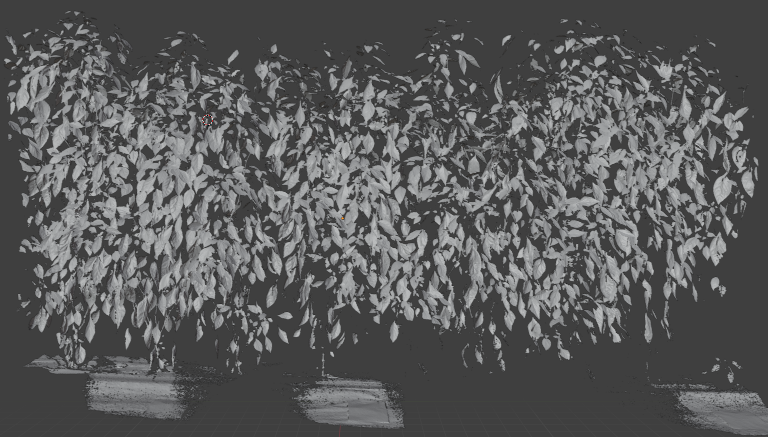
\includegraphics[width=110mm]{images/png/plant3d.png}
     \caption{3D model view}
     \label{Fig:plant3d}
   \end{figure}

\begin{table}[H]
  \begin{center}
    \begin{tabular}{l|p{30mm}p{30mm}p{30mm}c}
      ID & $d_fside$ [$mm$]& $d_fabove$ [$mm$]& $d_fbelow$ [$mm$]& $d_p$ [$mm$]\\ \hline\hline
      2 & 9.6 & - & 111.0 & 37.6\\
      4 & 12.9 & 18.3 & 38.5 & 2.8 \\
      5 & 12.4 & 18.9 & 1.5 & 2.3 \\
      7 & 107.0 & 54.9 & 152.1 & 70.5\\
      9 & 24.9 & 24.2 & 655.0 & 3.8\\
      10 & 12.9 & 24.0 & 32.4 & 2.3\\
      11 & 20.6 & 20.5 & 26.0 & 3.1\\
      13 & 20.5 & 22.7 & 728.1 & 2.5\\
      14 & 23.9 & 22.7 & 207.3 & 1.7\\
      20 & 9.6 & 25.9 & 24.1 & 1.2\\
      22 & 73.2 & 52.0 & 251.2 & 61.2\\
      30 & 18.6 & 52.8 & 1176.2 & 18.3\\
    \end{tabular}
    \caption{Measurement results① Obstacle distance}
    \label{Tab:measurementresults1}
  \end{center}
\end{table}

\begin{table}[H]
  \begin{center}
    \begin{tabular}{l|p{30mm}p{30mm}cc}
      ID & $S_f$ [$mm^2$] & $S_p$ [$mm^2$] & Peduncle width [$mm$] & Fruit width [$mm$]\\ \hline\hline
      2 & 767.0 & 124.7 & 20.8 & 6.4\\
      4 & 386.5 & 22.0 & 22.8 & 3.0\\
      5 & 299.0 & 23.0 & 26.4 & 4.6\\
      7 & 1827.7 & 85.1 & 33.4 & 3.5\\
      9 & 1201.6 & 109.3 & 28.2 & 4.5\\
      10 & 708.9 & 32.6 & 21.2 & 3.3\\
      11 & 604.6 & 18.6 & 18.1 & 3.0\\
      13 & 843.1 & 41.3 & 35.8 & 4.5\\
      14 & 949.6 & 19.6 & 24.7 & 2.9\\
      20 & 0.0 & 10.6 & 18.0 & 2.9\\
      22 & 1384.6 & 63.6 & 31.0 & 3.7\\
      30 & 924.8 & 53.3 & 21.9 & 4.0\\
    \end{tabular}
    \caption{Measurement results② Projected area and Width}
    \label{Tab:measurementresults2}
  \end{center}
\end{table}

\figref{Fig:resultbesidef} \verb|〜| \figref{Fig:resultbesidep} は各障害物間距離の分布を表すためのヒストグラムである.
グラフより, 果実下面障害物間距において60mm以上の割合が大きいことがわかるため, 果実の下方向はある程度空間があり, 果実にアプローチする場合は下方向からのアプローチが適しているのではないかと考えられる.
また, 果実側面障害物間距離に比べて, 花柄側面障害物間距離の15mm未満の割合が高くなっているが, これは花柄と果実の内部を含まずに中心から計測しているため, 花柄の幅と果実の幅の差が影響していると考えられる.

\vspace{5mm}
\begin{figure}[H]
     \centering
     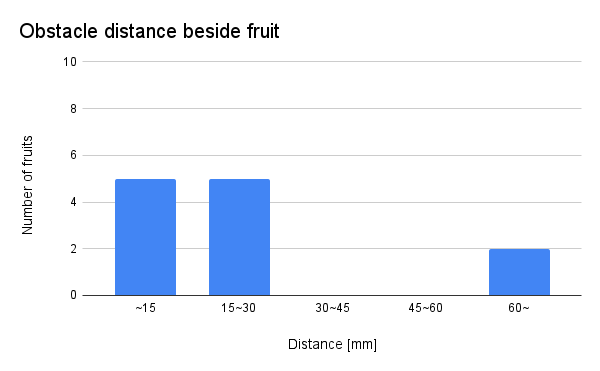
\includegraphics[width=110mm]{images/png/resultbesidef.png}
     \caption{Distribution of Obstacle distance beside fruit}
     \label{Fig:resultbesidef}
\end{figure}

\begin{figure}[H]
  \centering
  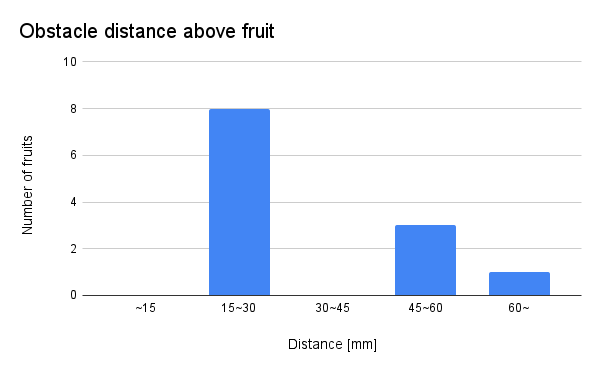
\includegraphics[width=110mm]{images/png/resultabovef.png}
  \caption{Distribution of Obstacle distance above fruit}
  \label{Fig:resultabovef}
\end{figure}

\begin{figure}[H]
  \centering
  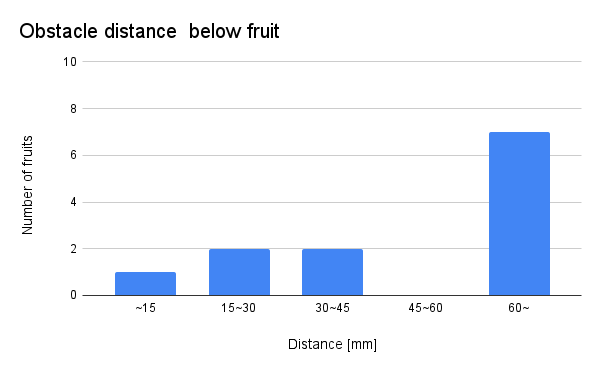
\includegraphics[width=110mm]{images/png/resultbelowf.png}
  \caption{Distribution of Obstacle distance below fruit}
  \label{Fig:resultbelowf}
\end{figure}

\begin{figure}[H]
  \centering
  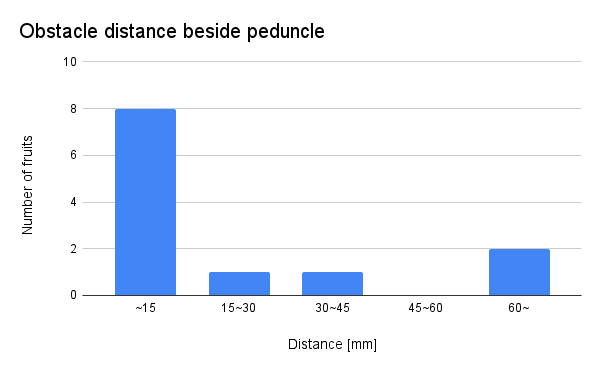
\includegraphics[width=110mm]{images/png/resultbesidep.png}
  \caption{Distribution of Obstacle distance beside peduncle}
  \label{Fig:resultbesidep}
\end{figure}

%花柄と果実の側面障害物間距離からそれぞれの幅の半分の値を引いたものと